\documentclass[a4paper,11pt]{article}
\usepackage[T1]{fontenc}
\usepackage[utf8]{inputenc}
\usepackage{lmodern}
\usepackage[english]{babel}
\usepackage{subcaption}
\usepackage{graphicx}
\usepackage{listings}
\usepackage{color}
\usepackage{hyperref}

\definecolor{dkgreen}{rgb}{0,0.6,0}
\definecolor{gray}{rgb}{0.5,0.5,0.5}
\definecolor{mauve}{rgb}{0.58,0,0.82}

\lstset{frame=tb,
  language=Python,
  aboveskip=3mm,
  belowskip=3mm,
  showstringspaces=false,
%   columns=flexible,
  basicstyle={\small\ttfamily},
  numbers=left,
%   frame=single,
  morekeywords={mean,std},
  numberstyle=\tiny\color{gray},
  keywordstyle=\color{blue},
  commentstyle=\color{dkgreen},
  stringstyle=\color{mauve},
  breaklines=true,
  breakatwhitespace=true,
  tabsize=3
}

\title{Computer vision - Homework 1}
\author{Nicolas Six}

\begin{document}

\maketitle

\section{Question 1}
\paragraph{}
The two images I chose for this homework are represented on Figure \ref{tree} and \ref{lena}

\begin{figure}[h!]
  \begin{center}
    \begin{subfigure}[t]{0.45\textwidth}
      \centering
      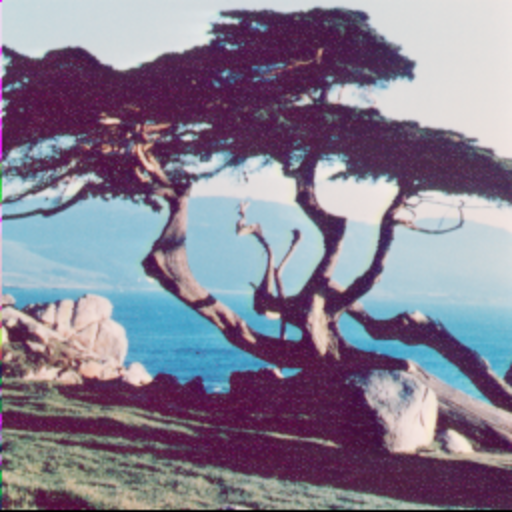
\includegraphics[width=0.9\linewidth]{Images/ps0-1-a-1.png}
      \caption{Tree}
      \label{tree}
    \end{subfigure}
    \begin{subfigure}[t]{0.45\textwidth}
      \centering
      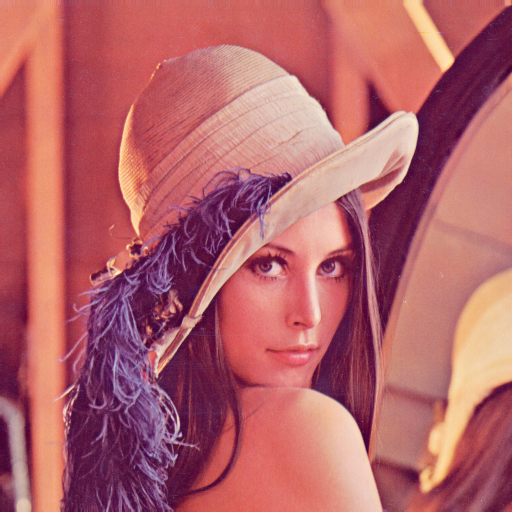
\includegraphics[width=0.9\linewidth]{Images/ps0-1-a-2.png}
      \caption{Lena}
      \label{lena}
    \end{subfigure}
  \end{center}
\end{figure}

\section{Question 2}

\paragraph{}
My answer for the part a, b and c of this question are displayed on Figures \ref{q2a}, \ref{q2b} and \ref{q2c} respectively.

\paragraph{}
The monochrome produced by the red channel of the source image is, to my mind, the clossest one to a monochromatic version of the source image on Figure \ref{tree}. The difference between the Figures \ref{q2b} and \ref{q2c} show us that the three different layers: red, green and blue, have not the same importance for an human viewer. Thus, that difference must be taken into account when using computer vision algorithm. But we can't say that a computer vision algorithm will perform better on one image than the other. For example, if you want to get precisely the tree position, the best is to use the green one, but if you want the mountain on the background the red is better than the green.

\begin{figure}[h!]
  \begin{center}
    \begin{subfigure}[t]{0.3\textwidth}
      \centering
      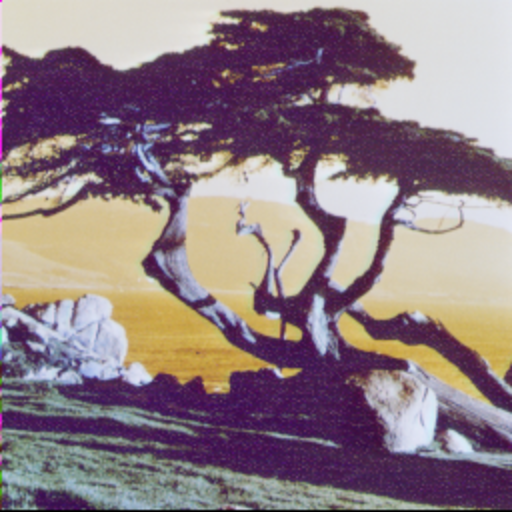
\includegraphics[width=0.9\linewidth]{Images/ps0-2-a.png}
      \caption{Tree with the value for the red and blue pixels swapped}
      \label{q2a}
    \end{subfigure}
    \begin{subfigure}[t]{0.3\textwidth}
      \centering
      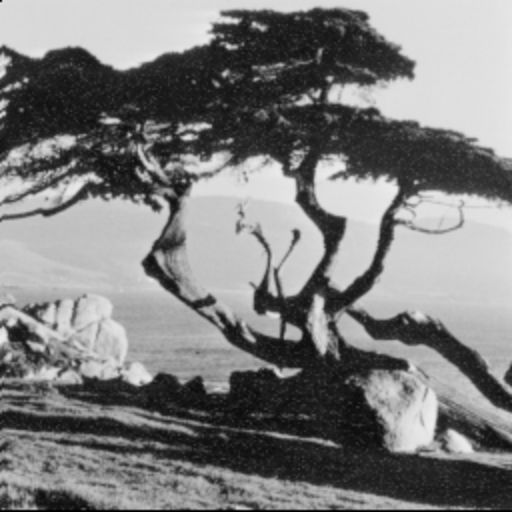
\includegraphics[width=0.9\linewidth]{Images/ps0-2-b.png}
      \caption{Tree with the green channel values set to the three different channels}
      \label{q2b}
    \end{subfigure}
    \begin{subfigure}[t]{0.3\textwidth}
      \centering
      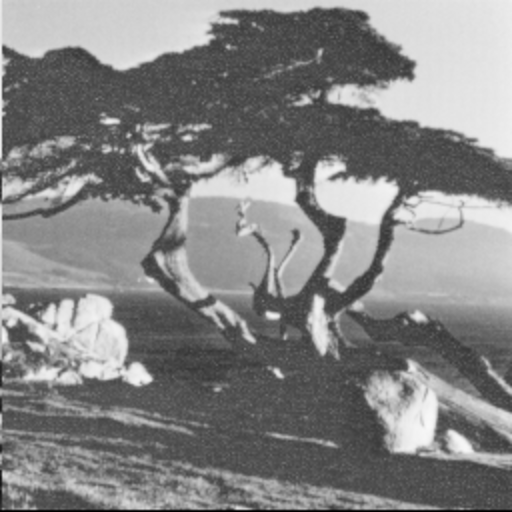
\includegraphics[width=0.9\linewidth]{Images/ps0-2-c.png}
      \caption{Tree with the red channel values set to the three different channels}
      \label{q2c}
    \end{subfigure}
  \end{center}
\end{figure}

\section{Question 3}

\begin{figure}[h!]
  \centering
  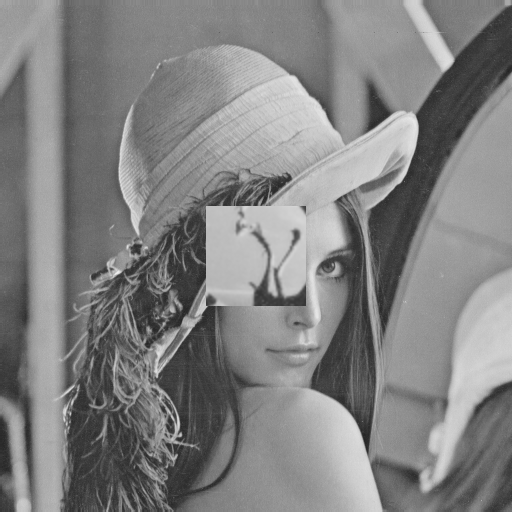
\includegraphics[width=0.5\linewidth]{Images/ps0-3.png}
  \caption{Lena with a patch of 100x100 pixels from the Tree in the center of the image}
  \label{q3}
\end{figure}

\section{Question 4}
\paragraph{}
In the Python code I used the image as read by OpenCV are stored as numPy array. The minimum, maximum, mean and standard deviation are then easy to get using the corespondent numPy functions, as you can see on the following code.

\begin{lstlisting}
# gt being the matrix with the values
# from the green layer of the tree image
print("max: ", np.max(gt))
print("min: ", np.min(gt))
print("mean:", np.mean(gt))
print("std: ", np.std(gt))
\end{lstlisting}

\paragraph{}
Once run this part of the code give the following output:

\begin{lstlisting}
max:  237
min:  0
mean: 124.906745911
std:  75.6626451933  
\end{lstlisting}

\begin{figure}[h!]
  \begin{center}
    \begin{subfigure}[t]{0.3\textwidth}
      \centering
      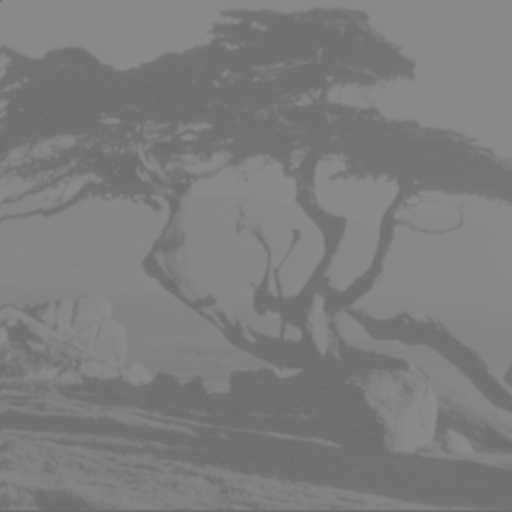
\includegraphics[width=0.9\linewidth]{Images/ps0-4-b.png}
      \caption{Image of the Tree green layer after multiple computations, some of them involving overflow of the tiny uint8 where they are stored}
      \label{q4b}
    \end{subfigure}
    \begin{subfigure}[t]{0.3\textwidth}
      \centering
      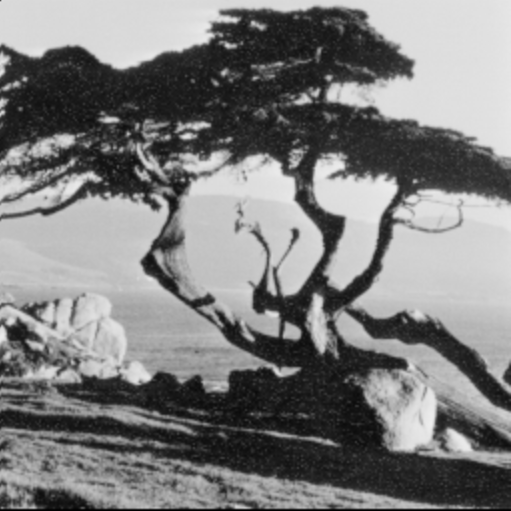
\includegraphics[width=0.9\linewidth]{Images/ps0-4-c.png}
      \caption{Tree image shifted by two pixels to the right}
      \label{q4c}
    \end{subfigure}
    \begin{subfigure}[t]{0.3\textwidth}
      \centering
      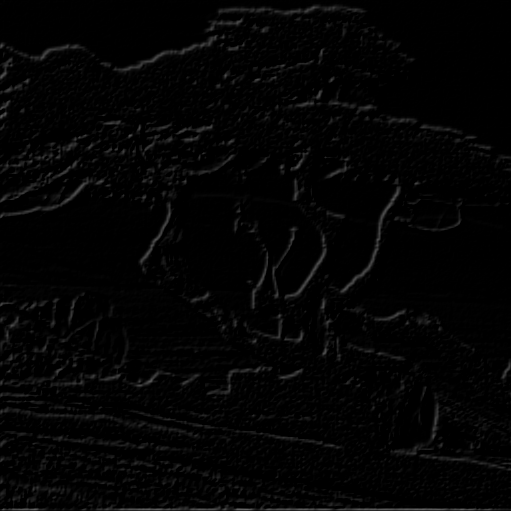
\includegraphics[width=0.9\linewidth]{Images/ps0-4-d.png}
      \caption{Subtraction of the original image by the two pixels shifted image, also known as the horizontal derivative (negative pixel don't mean anything, that's why they are coded on unsigned 8 bits integer. That being said overflow can give quite beautiful images)}
      \label{q4d}
    \end{subfigure}
  \end{center}
\end{figure}

\section{Question 5}
\paragraph{}
Figure \ref{q5a} and \ref{q5b} represent the Tree image with an added Gaussian noise on the green and blue layer respectively. Even if a noise with the same property is applied to the two images, the result is completely different to the human eye. This is probably due to the fact that the human eye is more sensitive to the green than the blue as you can see on Figure \ref{vision}. If we call the Earth the blue planet, our eyes evolved in the mostly green environment of inland landscape and particularly forest where being able to distinguish a large number of green can some times increase the odd of survival. The Blue is, in that situation far less important, it's mostly a heritage from our maritime ancestor and is, far less sensitive. The red on his part is just an extra and is not seen very well neither, but contrast well on the green and is so easy to spot.

\begin{figure}
  \centering
  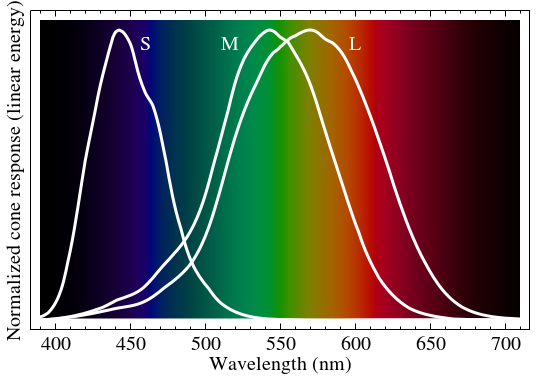
\includegraphics[width=0.5\linewidth]{vision.png}
  \caption{Sensibility of the three human color preceptor according to the wavelength \cite{wiki:vision}}
  \label{vision}
\end{figure}

\begin{figure}
  \begin{center}
    \begin{subfigure}[t]{\textwidth}
      \centering
      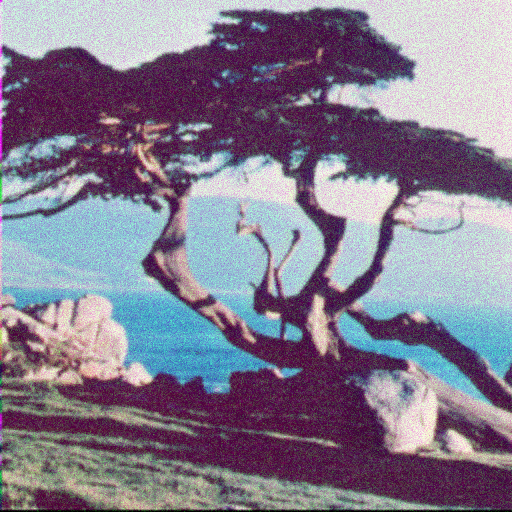
\includegraphics[width=0.8\linewidth]{Images/ps0-5-a.png}
      \caption{Tree with a Gaussian noise on the green layer ($sigma=25$)}
      \label{q5a}
    \end{subfigure}
    \begin{subfigure}[t]{\textwidth}
      \centering
      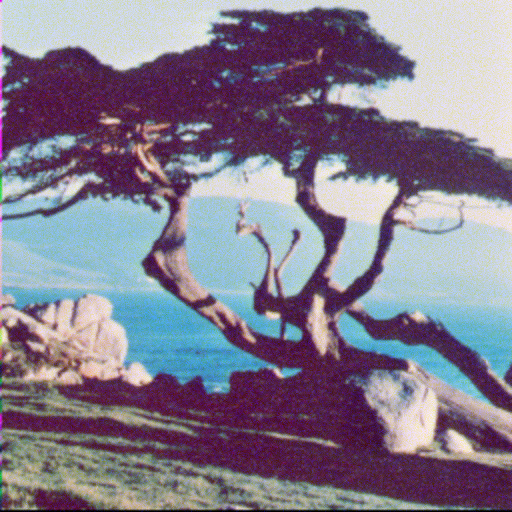
\includegraphics[width=0.8\linewidth]{Images/ps0-5-b.png}
      \caption{Tree with a Gaussian noise on the blue layer ($sigma=25$)}
      \label{q5b}
    \end{subfigure}
  \end{center}
\end{figure}

\bibliography{cv}{}
\bibliographystyle{plain}


\end{document}
